\documentclass{article}

% Russian language
\usepackage[utf8]{inputenc}
\usepackage[russian]{babel}

\usepackage{biblatex}       % for roman digits

\usepackage{amsmath, amssymb}
\usepackage[left=20mm, right=20mm, top=2cm]{geometry}
\usepackage{array}

\usepackage{graphicx}
\usepackage{ragged2e}
\usepackage{wrapfig}
\justifying

\graphicspath{{images/}}

\title{
    \textbf{Лабораторная работа 3.1.3}
}
\author{Герасименко Д.В.}
\date{2 курс ФРКТ, группа Б01-104}

\begin{document}

\maketitle

\begin{center}
    \raggedleft
        \underline{\underline{\LARGE {Аннотация}}}
\end{center}

\begin{center}
\raggedright
    \large{\textbf{Тема:}}
    \\
    \large {Измерение магнитного поля Земли}
    
    \large{\textbf{Цель работы:}}
    \\
    \large {Определить характеристики шарообразных неодимовых магнитов и, используя законы взаимодействия магнитных моментов с полем, измерить горизонтальную и вертикальную составляющие индукции магнитного поля Земли и магнитное наклонение.}
    
    \large{\textbf{Оборудование:}}
    \\
    \large{12 одинаковых неодимовых магнитных шариков, тонкая нить для изготовления крутильного маятника, медная проволока диаметром ($0,5 - 0,6$) мм, электронные весы, секундомер, измеритель магнитной индукции АТЕ-8702, штангенциркуль, брусок из немагнитного материала ($25\times30\times60$ мм$^3$), деревянная линейка, штатив из немагнитного материала; дополнительные неодимовые магнитные шарики ($\sim$ 20 шт.) набор гирь и разновесов.}
\end{center}

\begin{center}
    \raggedleft
        \underline{\underline{\LARGE {Теория}}}
\end{center}

\begin{center}
    \underline{\large {\RN{1}.Точечный магнитный диполь}}
\end{center}

Простейший магнитный диполь может быть образован витком с током или постоянным магнитом. По определению, магнитный момент $\vec{P_m}$ тонкого витка площадью $S$ с током $I$ равен:

\begin{equation}
    \vec{P_m} = \dfrac{I}{c}\vec{S} = \dfrac{I}{c} S \vec{n}
\end{equation} 
где $c$ – скорость света в вакууме, $\vec{S} = S \vec{n}$ — вектор площади контура, образующий с направлением тока правовинтовую систему, $\vec{n}$ --- единичный вектор нормали к площадке $S$ (это же направление $\vec{P}_m$ принимается за направление $S \to N$ от южного ($S$) к северному ($N$) полюсу). Если размеры контура с током или магнитной стрелки малы по сравнению расстоянием до диполя, то соответствующий магнитный диполь $\vec{P}_m$ называют элементарным или точечным.

Поле точечного диполя определяется по следующей формуле:

\begin{equation}
    \vec{B} = \dfrac{3\left(\vec{P_m}, \vec{r}\right)\vec{r}}{r^5} - \dfrac{\vec{P}_m}{r^3}
\end{equation}

В магнитном поле с индукцией $\vec{B}$ на точечный магнитный диполь $\vec{P}_m$ действует механический момент сил:

\begin{equation}
    \vec{M} = \left[\vec{P_m}, \vec{B}\right]
\end{equation}

Под действием вращающего момента $\vec{M}$ виток с током или постоянный магнит поворачивается так, чтобы его магнитный момент выстроился вдоль вектора индукции магнитного поля. Это --- положение устойчивого равновесия: при отклонении от этого положения возникает механический момент внешних сил, возвращающий диполь к положению равновесия. В положении, когда $\vec{P_m}$ и $\vec{B}$ параллельны, но направлены противоположно друг другу, также имеет место равновесие ($M = 0$), но такое равновесие неустойчиво: малейшее отклонение от этого положения приведёт к появлению момента сил, стремящихся отклонить диполь ещё дальше от начального положения.

Магнитный диполь в магнитном поле обладает энергией:

\begin{equation}
    W = -\left(\vec{P_m}, \vec{B}\right)
\end{equation}

\begin{center}
    \underline{\large {\RN{2}.{Неодимовые магниты}}}
\end{center}

В настоящей работе используются неодимовые магниты шарообразной формы.
Для нас важно то, что:
\begin{enumerate}
\item шары намагничены однородно;
\item вещество, из которого изготовлены магниты, является магнитожёстким материалом.
\end{enumerate}
Внутри такого шара магнитное поле равно 

\begin{equation}
    B_0 = \dfrac{2P_m}{R^3}
\end{equation}

Полный магнитный момент $\vec{P_m}$ постоянного магнита определяется намагниченностью $\vec{p_m}$ вещества, из которого он изготовлен. По определению, намагниченность --- это магнитный момент единицы объёма. Для однородно намагниченного шара намагниченность, очевидно, равна:

\begin{equation}
    \vec{p_m} = \dfrac{\vec{P_m}}{V}
\end{equation}

Намагниченность — важная характеристика вещества постоянных магнитов, определяющая, в частности, величину остаточной магнитной индукции $B_r = 4 \pi p_m$ (остаточная индукция $B_r$ --- одна из величин, которая, как правило, указывается в справочниках по магнитожёстким материалам).

\begin{equation}
    \vec{B_P} = \dfrac{8\pi}{3}\vec{p_m} = \dfrac{2}{3} \vec{B_r}
\end{equation}

\begin{center}
    \underline{\large {\RN{3}.{Экспериментальное определение величины магнитного момента магнитных шариков}}}
\end{center}

$P_m$ можно определить из параметров шарика и из расстояния $r_{max}$, на котором они удерживаются в поле тяжести.

\begin{equation}
    P_m = \sqrt{\dfrac{mgr_{max}^4}{6}}
\end{equation}

\begin{equation}
    \vec{B_p} = \dfrac{2\vec{P_m}}{R^3}
\end{equation}

\begin{center}
    \underline{\large {\RN{4}.{Определение величины магнитного момента по силе сцепления магнитных шариков}}}
\end{center}

Если сила сцепления двух одинаковых шаров равна 

\begin{equation}
    F_0 = \dfrac{6P_m^2}{d^4} \Rightarrow P_m = \sqrt{\dfrac{F_0d^4}{6}}
\end{equation}
то минимальный вес цепочки, при которой она оторвется от верхнего шарика равен:

\begin{equation}
    F \approx 1,08F_0
\end{equation}

\begin{center}
    \underline{\large {\RN{5}.{Измерение горизонтальной составляющей индукции магнитного поля Земли}}}
\end{center}

\begin{center}
    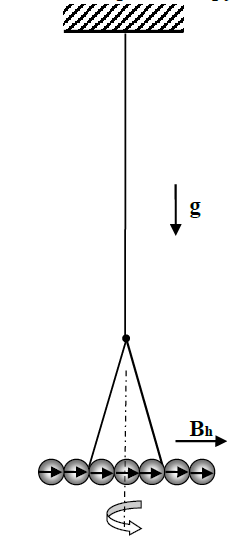
\includegraphics[width = 0.2\textwidth]{Bhor.png}
    
    \textbf{Рис.1.} Критильный маятник
\end{center}

При отклонении "стрелки" на угол $\theta$ от равновесного положения в горизонтальной плоскости возникают крутильные колебания вокруг вертикальной оси, проходящей через середину стрелки. Если пренебречь упругостью нити, то уравнение крутильных колебаний такого маятника определяется возвращающим моментом сил $M = -P_0B_h \sin \theta$, действующим на "стрелку" со стороны магнитного поля Земли, и моментом инерции $I_n$ "стрелки" относительно оси вращения.\\
При малых амплитудах:

\[T = 2\pi \sqrt{\dfrac{I_n}{nP_mB_h}}\]
Пусть 
\[T(n) = kn \Rightarrow\]

\begin{equation}
    k = \pi \sqrt{\dfrac{md^2}{3P_m B_h}} \Rightarrow B_h = \dfrac{\pi^2md^2}{3k^2P_m}
\end{equation}

\begin{center}
    \underline{\large {\RN{6}.{Измерение вертикальной составляющей индукции магнитного поля Земли.}}}
\end{center}

С помощью небольшого дополнительного грузика "стрелку" можно "выровнять", расположив её горизонтально: в этом случае момент силы тяжести груза относительно точки подвеса будет равен моменту сил, действующих на "стрелку" со стороны магнитного поля Земли. Если масса уравновешивающего груза равна $m$, плечо силы тяжести $r$, а полный магнитный момент "стрелки" $P_0 = nP_m$, то в равновесии:
\[
    mgr = P_0 B_v = nP_mB_v
\]

\begin{equation}
    B_v = \dfrac{M(n)}{P_m}
\end{equation}

\begin{center}
    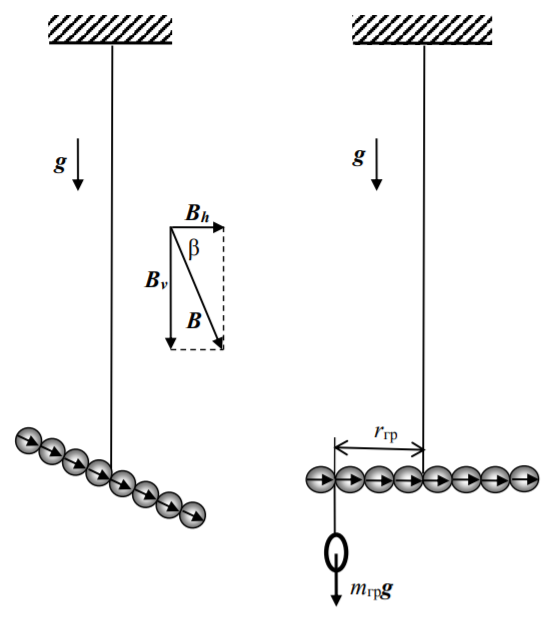
\includegraphics[width=0.5\textwidth]{Bver.png}
\end{center}

\begin{center}
    \raggedleft
        \underline{\underline{\LARGE {Выполнение}}}
\end{center}

\begin{center}
    \underline{\large {\RN{1}.Определение магнитного момента, намагниченности и остаточной магнитной индукции шариков}}
\end{center}

\subsubsection*{Метод A. }

Возьмем 8 неодимовых шариков, измерим их массы и диаметры с помощью электронных весов и микрометра. 
Определим средние параметры наших шариков и запишем их в таблицу.

\begin{center}
    \begin{tabular}{|c|c|c|}
        \hline
        Параметр & Значение & $\sigma$ \\
        \hline
        $m$, г & 0.833 & 0.001 \\
        \hline
        $d$, мм & 5.91 & 0.01 \\
        \hline
    \end{tabular}
    
    \textbf{Таблица 1.} Параметры шариков.
\end{center}

Определим $r_{max}$. Затем по формуле $(8)$ определим $P_m$, по формуле $(6)$ определим $p_m$, по формуле $(9)$ определим $B_p$ и по формуле $(7)$ определим $B_r$. Все полученные данные занесем в таблицу 2.

\begin{center}
    \begin{tabular}{|c|c|c|}
        \hline
        Величина & Значение в СГС & Значение в СИ \\
        \hline
        $r_{max}$ & \(1.47 \pm 0.01\) см & \((1.47 \pm 0.01)\) см \\
        \hline
        $P_m$ & \((25.2 \pm 0.7) \cdot 10^{-6} \frac{\text{эрг}}{\text{Гс}}\), $\cdot$ см$^3$ & \((7.97 \pm 0.22), 10^{-6} \text{A} \cdot \text{м}^{2}\)\\
        \hline
        $p_m$ & \((233 \pm 7)\), Гс & \((74 \pm 2)\), Тл \\
        \hline
        $B_p$ & \((1.95 \pm 0.06)\), кГс & \((617 \pm 17)\), Тл \\
        \hline
        $B_r$ & \((2.93 \pm 0.08)\), кГс & \((925 \pm 26)\), Тл \\
        \hline
    \end{tabular}
    
    \textbf{Таблица 2.} Величины, определяемые в методе А.
\end{center}

Меряем $B_p$ с помощью магнитометра и получаем $B_p = (275 \pm 5)$ мТл.

\subsubsection*{Метод B}

Составим цепочку и определим $F$ - вес грузиков, которые надо подвесить к этой цепочке, чтобы грузики оторвались. 

По формуле $(11)$ определим силу сцепления двух шаров. По формуле $(10)$ найдем $P_m$ и запишем все данные в таблицу.

\begin{center}
    \begin{tabular}{|c|c|c|}
    \hline
        Величина & Значение в СГС & Значение в СИ\\
        \hline
        $M$ & \((327 \pm 10)\), г & \((327 \pm 10) \cdot 10^{-3}\), кг \\
        \hline
        $F$ & \((3.20 \pm 0.09) \cdot 10^{5}\), дин & \((3.20 \pm 0.09) \), Н \\
        \hline
        $F_0$ & \((2.97 \pm 0.08) \cdot 10^{5}\), дин & \((2.97 \pm 0.08)\), Н \\
        \hline
        $P_m$ & \((77.7 \pm 4.7), \frac{\text{эрг}}{\text{Гс}}\) & \((24.5 \pm 1.5), 10^{-6} \text{A} \cdot \text{м}^{2}\) \\
        \hline
    \end{tabular}
    
    \textbf{Таблица 3.} Величины, определяемые в методе B.
\end{center}

В итоге получаем, что $P_m = (77.7 \pm 4.7) \frac{\text{эрг}}{\text{Гс}}$. $B_p = (6.1 \pm 0.4)$ кГс, а $B_r = (9.1 \pm 0.2) $ кГс, что очень близко к табличным значениям ($1.03 - 1.13$ кГс), но довольно далеко от измеренного нами поля магнитометром.

В дальнейших этапах выполнения в качестве магнитного момента шарика будем использовать значение, получившееся из непосредственного измерения с помощью магнитометра:

\[
    P_{m} = (37.2 \pm 0.1) \frac{\text{эрг}}{\text{Гс}} 
\]

\begin{center}
    \underline{\large {\RN{2}.Определение горизонтальной составляющей магнитного поля Земли}}
\end{center}

Для определения горизонтальной составляющей магнитного поля Земли нам нужно собрать установку для возбуждения крутильных колебаний и исследовать зависимость количество шариков от периода. 

Перед этим удостоверимся, что при расчете периода упругость нити можно не учитывать, свернув стрелку в кольцо и измерив период крутильных колебаний (очевидно, что магнитный момент такой стрелки равен 0).

Получаем $T = 54$ с. Это означает, что мы можем пренебречь упругостью нитей.

\begin{center}
    \begin{tabular}{|c|c|}
        \hline
        $n$ & $T$, с \\
        \hline
        12 & 2.901 \\
        \hline
        11 &  2.652 \\
        \hline
        10 & 2.441 \\
        \hline
        9 & 2.189 \\
        \hline
        8 & 1.925 \\
        \hline
        7 & 1.681 \\
        \hline
        6 & 1.423 \\
        \hline
        5 & 1.174 \\
        \hline
        4 & 0.975 \\ 
        \hline
        3 & 0.724 \\
        \hline
    \end{tabular}
    
    \textbf{Таблица 4. } Зависимость крутильных колебаний от количества шариков $T(n)$
\end{center}

Построим график зависимости $T(n)$ и по формуле $(12)$ найдем $B_h$.

По значению углового коэффициента $k$ рассчитаем величину горизонтальной составляющей магнитного поля Земли по формуле $(8)$.
\[
    B_h = (205 \pm 17) \text{Гс}
\]

\newpage

\begin{center}
    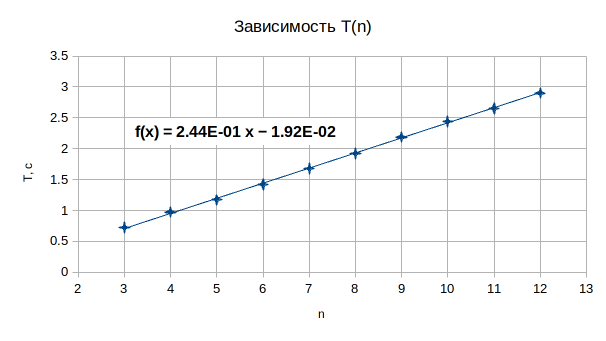
\includegraphics[width=0.7\textwidth]{T(n).png}
    
    \textbf{Рис. 1.} График зависимости T(n)
\end{center}

\begin{center}
    \underline{\large {\RN{3}.Определение вертикальной составляю-щей магнитного поля Земли}}
\end{center}

Определяем механический момент сил, действующий со стороны магнитного поля Земли на горизонтально расположенную магнитную "стрелку". Для этого, с помощью одного или нескольких кусочков проволоки, уравновесьте "стрелку" в горизонтальном положении. Сделаем измерения для разных количеств шариков и занесем все в таблицу.

\begin{center}
    \begin{tabular}{|c|c|c|c|}
        \hline
        $n$ & $M$, дин$\cdot$см \\ \hline
        12 & 194.5 \\
        \hline
        10 & 167.7 \\
        \hline
        8 & 138.3 \\
        \hline
        6 & 101.8 \\
        \hline
        4 & 59.5 \\
        \hline
    \end{tabular}
    
    \textbf{Таблица 5.} Зависимость момента сил от $n$.
\end{center}

\begin{center}
    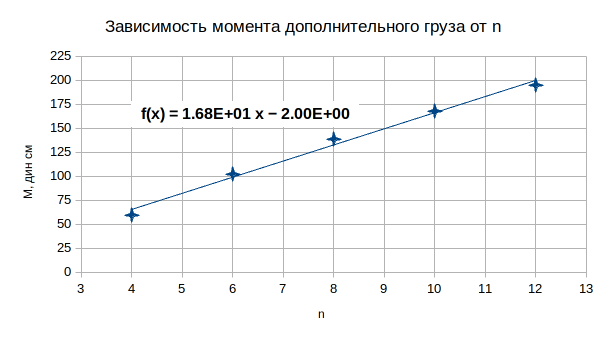
\includegraphics[width=0.7\textwidth]{M(n).png}
    
    \textbf{Рис. 2.} График зависимости M(n)
\end{center}

По формуле $(13)$ определяем $B_v = (453 \pm 21)$ Гс.

В итоге получаем, что $B = (0.495 \pm 0.025)$ мТл и $\beta = (66 \pm 3)^{\circ}$, что очень близко к современным данным в нашем регионе.

\begin{center}
    \raggedleft
        \underline{\underline{\LARGE {Вывод}}}
\end{center}

\begin{center}
    \LARGE{НАПЛОДИТЬ ВЫВОД}
\end{center}

\end{document}
